\chapter{Mantener y cambiar la librería}\label{cap:mantenimiento}

Una librería compartida solo funciona si los cambios se hacen con orden. Este capítulo explica cómo se cambia y cómo se reparte una versión nueva.

\section{Cuándo cambiar la librería (y cuándo no)}
\begin{itemize}
\item \textbf{Sí}: hay un fallo; hay una necesidad que comparten varias estaciones.
\item \textbf{No}: algo que solo necesita tu estación (va en tu aplicación); un cambio de significado de un byte del tag (va en el Excel y en tus constantes).
\end{itemize}

\section{Cómo se pide un cambio}
Se manda al grupo (y a quien mantiene la librería): qué ocurre, en qué estación y con qué versión, y qué propones. Si es un fallo, el material del capítulo~\ref{cap:problemas}, «si nada de esto sirve». No se corrige en el proyecto de cada uno: no se puede, y si se pudiera, las estaciones dejarían de ser iguales.

\section{Cómo se hace un cambio}
Lo hace una sola persona, en la librería:

\reiniciapaso
\paso{Edita el tipo en la librería}
En el panel de librerías, abre el tipo (por ejemplo, \cod{Est\_FB\_Estacion}) para editarlo. La librería exige que se edite el \emph{tipo}, no la copia que hay en un proyecto.

\paso{Prueba el cambio}
Compila. Después, ejecuta las pruebas del simulador de la librería (capítulo~\ref{cap:pruebas}) si las tienes, o las de aceptación del grupo.

\paso{Asigna una versión nueva}
Con \menu{Assign version} (Asignar versión) sobre el tipo, dale un número nuevo. La versión de un tipo ya asignada no se puede modificar: cualquier arreglo es una versión nueva.

\paso{Archiva la librería}
En el panel de librerías, clic derecho sobre \menu{CPLabCore} y \menu{Archive library...} (Archivar librería). Elige el formato comprimido (\texttt{.zal20}) y el nombre con la versión: \texttt{CPLabCore\_v1.0.2.zal20}.

\begin{figure}[ht]
\centering
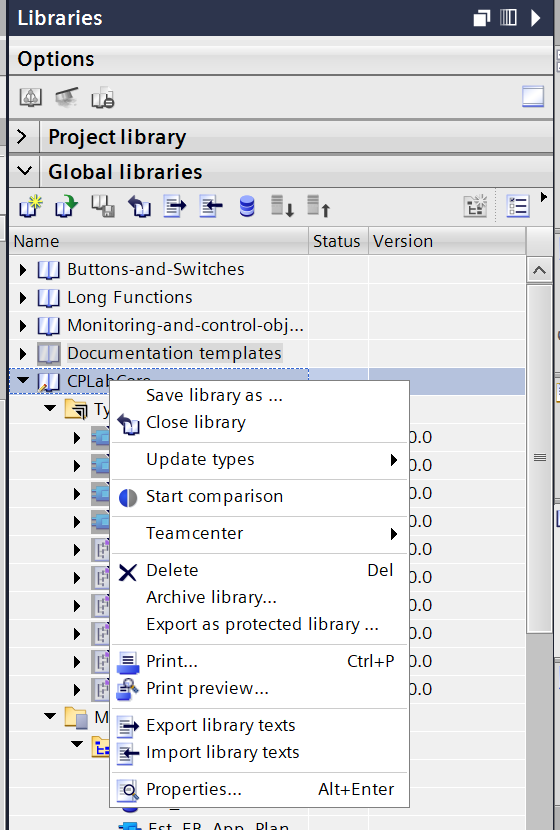
\includegraphics[width=0.55\textwidth]{capturas/menu_biblioteca.png}
\caption{El menú de la librería: \menu{Archive library...}, \menu{Update types}, \menu{Save library as...} y otros.}
\end{figure}

\paso{Avisa al grupo}
Con el nuevo archivo, qué cambia, y si hace falta cambiar algo en \cod{Main} o en las aplicaciones.

\section{Numeración de versiones}
\begin{center}
\small
\begin{tabularx}{\textwidth}{>{\bfseries}p{2.8cm}p{2.8cm}X}
\toprule
Cambio & Se incrementa & Ejemplo \\
\midrule
Arreglo de un fallo, sin cambiar pines & el último número & 1.0.1 $\rightarrow$ 1.0.2 \\
Función nueva compatible (pines nuevos con valor por defecto) & el segundo & 1.0.2 $\rightarrow$ 1.1.0 \\
Cambio incompatible (pines quitados, otro formato) & el primero & 1.1.0 $\rightarrow$ 2.0.0 \\
\bottomrule
\end{tabularx}
\end{center}
Una versión de «arreglo» se puede actualizar sin pensar; una «compatible» también, pero no hace falta usar lo nuevo; una «incompatible» exige revisar \cod{Main} y las aplicaciones.

\section{Registro de cambios}
\begin{center}
\small
\begin{tabularx}{\textwidth}{>{\bfseries}p{1.6cm}p{2.7cm}X}
\toprule
Versión & Fecha & Cambios \\
\midrule
1.0.1 & 12/11/2026 & Corrige un error en \cod{Est\_FB\_Estacion}: la condición que apaga la cinta estaba invertida (\cod{IF NOT Inhibir\_cinta} pasa a \cod{IF Inhibir\_cinta}) y la cinta no arrancaba nunca. \\
1.0.0 & 12/11/2026 & Primera versión: \cod{Est\_FB\_Estacion}, \cod{Est\_FB\_Modo}, \cod{Est\_FB\_Cinta}, \cod{Est\_FB\_RFID} y los seis UDT, con la imagen de 28 bytes, las máscaras y las direcciones. \textbf{No usar: error de la cinta.} \\
\bottomrule
\end{tabularx}
\end{center}

\section{Mejoras que se pueden plantear}
Cosas que se han visto al hacer la librería y que mejorarían una versión futura (el apéndice~\ref{ap:abiertos} las detalla):
\begin{itemize}
\item Que la librería lea siempre la unión de la máscara de lectura y la de escritura, para eliminar la regla de oro O1.
\item Un tiempo máximo para la aplicación, con aviso, para que una aplicación atascada no bloquee la estación.
\item Quitar la etapa de la cinta que no se usa.
\item Revisar con el hardware real la polaridad del sensor del stopper.
\end{itemize}
